\let\negmedspace\undefined
\let\negthickspace\undefined
\documentclass[journal]{IEEEtran}
\usepackage[a4paper, margin=10mm, onecolumn]{geometry}
%\usepackage{lmodern} % Ensure lmodern is loaded for pdflatex
\usepackage{tfrupee} % Include tfrupee package

\setlength{\headheight}{1cm} % Set the height of the header box
\setlength{\headsep}{0mm}  % Set the distance between the header box and the top of the text

\usepackage{gvv-book}
\usepackage{gvv}
\usepackage{cite}
\usepackage{amsmath,amssymb,amsfonts,amsthm}
\usepackage{algorithmic}
\usepackage{graphicx}
\usepackage{float}
\usepackage{textcomp}
\usepackage{xcolor}
\usepackage{txfonts}
\usepackage{listings}
\usepackage{enumitem}
\usepackage{mathtools}
\usepackage{gensymb}
\usepackage{comment}
\usepackage[breaklinks=true]{hyperref}
\usepackage{tkz-euclide} 
\usepackage{listings}
% \usepackage{gvv}                                        
\def\inputGnumericTable{}                                 
\usepackage[latin1]{inputenc}                                
\usepackage{color}                                            
\usepackage{array}                                            
\usepackage{longtable}                                       
\usepackage{calc}                                             
\usepackage{multirow}                                         
\usepackage{hhline}                                           
\usepackage{ifthen}                                           
\usepackage{lscape}
\usepackage{tikz}
\usetikzlibrary{patterns}

\begin{document}

\bibliographystyle{IEEEtran}
\vspace{3cm}

\title{8.2.31}
\author{ee25btech11063-vejith}

\maketitle
% \maketitle
% \newpage
% \bigskip
{\let\newpage\relax\maketitle}
\renewcommand{\thefigure}{\theenumi}
\renewcommand{\thetable}{\theenumi}
\setlength{\intextsep}{10pt} % Space between text and floats
\textbf{Question}\\
Find the equation of conic if ends of the major axis are \brak{\pm 3,0} and ends of the minor axis are  \brak{0,\pm 2}\\
\textbf{solution}\\
The equation of conic is represented as
\begin{align}
\vec{x}^\top\vec{V}\vec{x} + 2\vec{u}^\top\vec{x} + f = 0\\
\vec{V}=\norm{\vec{n}}^2\vec{I}-e^2\vec{n}\vec{n}^\top
\end{align}
As the major axis is along the X-axis 
\begin{align}
    \vec{n}=\vec{e_1}\\
    \implies \vec{V}=\begin{pmatrix}
        1-e^2 & 0\\
        0 & 1
    \end{pmatrix}
\end{align}
as the centre of ellipse is $\vec{c}$= $\vec{0}$
\begin{align}
    \implies \vec{u}=\vec{0}
\end{align}
let
\begin{align}
    \vec{P}=\myvec{0\\2}
\end{align}
$\vec{P}$  satisfy (1)
\begin{align}
    \vec{P}^\top\vec{V}\vec{P} + 2\vec{u}^\top\vec{P} + f = 0\\
    \brak{0\hspace{0.5cm} 2} \begin{pmatrix}
        1-e^2 & 0\\
        0 & 1
    \end{pmatrix}\myvec{0\\2} +f=0\\
     4+f=0 \\
     \implies f=-4
\end{align}
End of the ellipse $\myvec{3\\0}$ also satisfy (1)
\begin{align}
    \brak{3\hspace{0.5cm} 0} \begin{pmatrix}
        1-e^2 & 0\\
        0 & 1
    \end{pmatrix}\myvec{3\\0} +f=0\\
    \implies 9\brak{1-e^2}+f=0
\end{align}
from (10)
\begin{align}
    1-e^2=\frac{4}{9}\\
    \implies e^2=\frac{5}{9}\\
    \implies \vec{V}= \begin{pmatrix}
        \frac{4}{9} & 0\\
        0 & 1
    \end{pmatrix}
\end{align}
Equation of conic is 
\begin{align}
   \vec{x}^\top \begin{pmatrix}
        \frac{4}{9} & 0\\
        0 & 1
    \end{pmatrix} \vec{X}-4=0
\end{align}

\begin{figure}
    \centering
    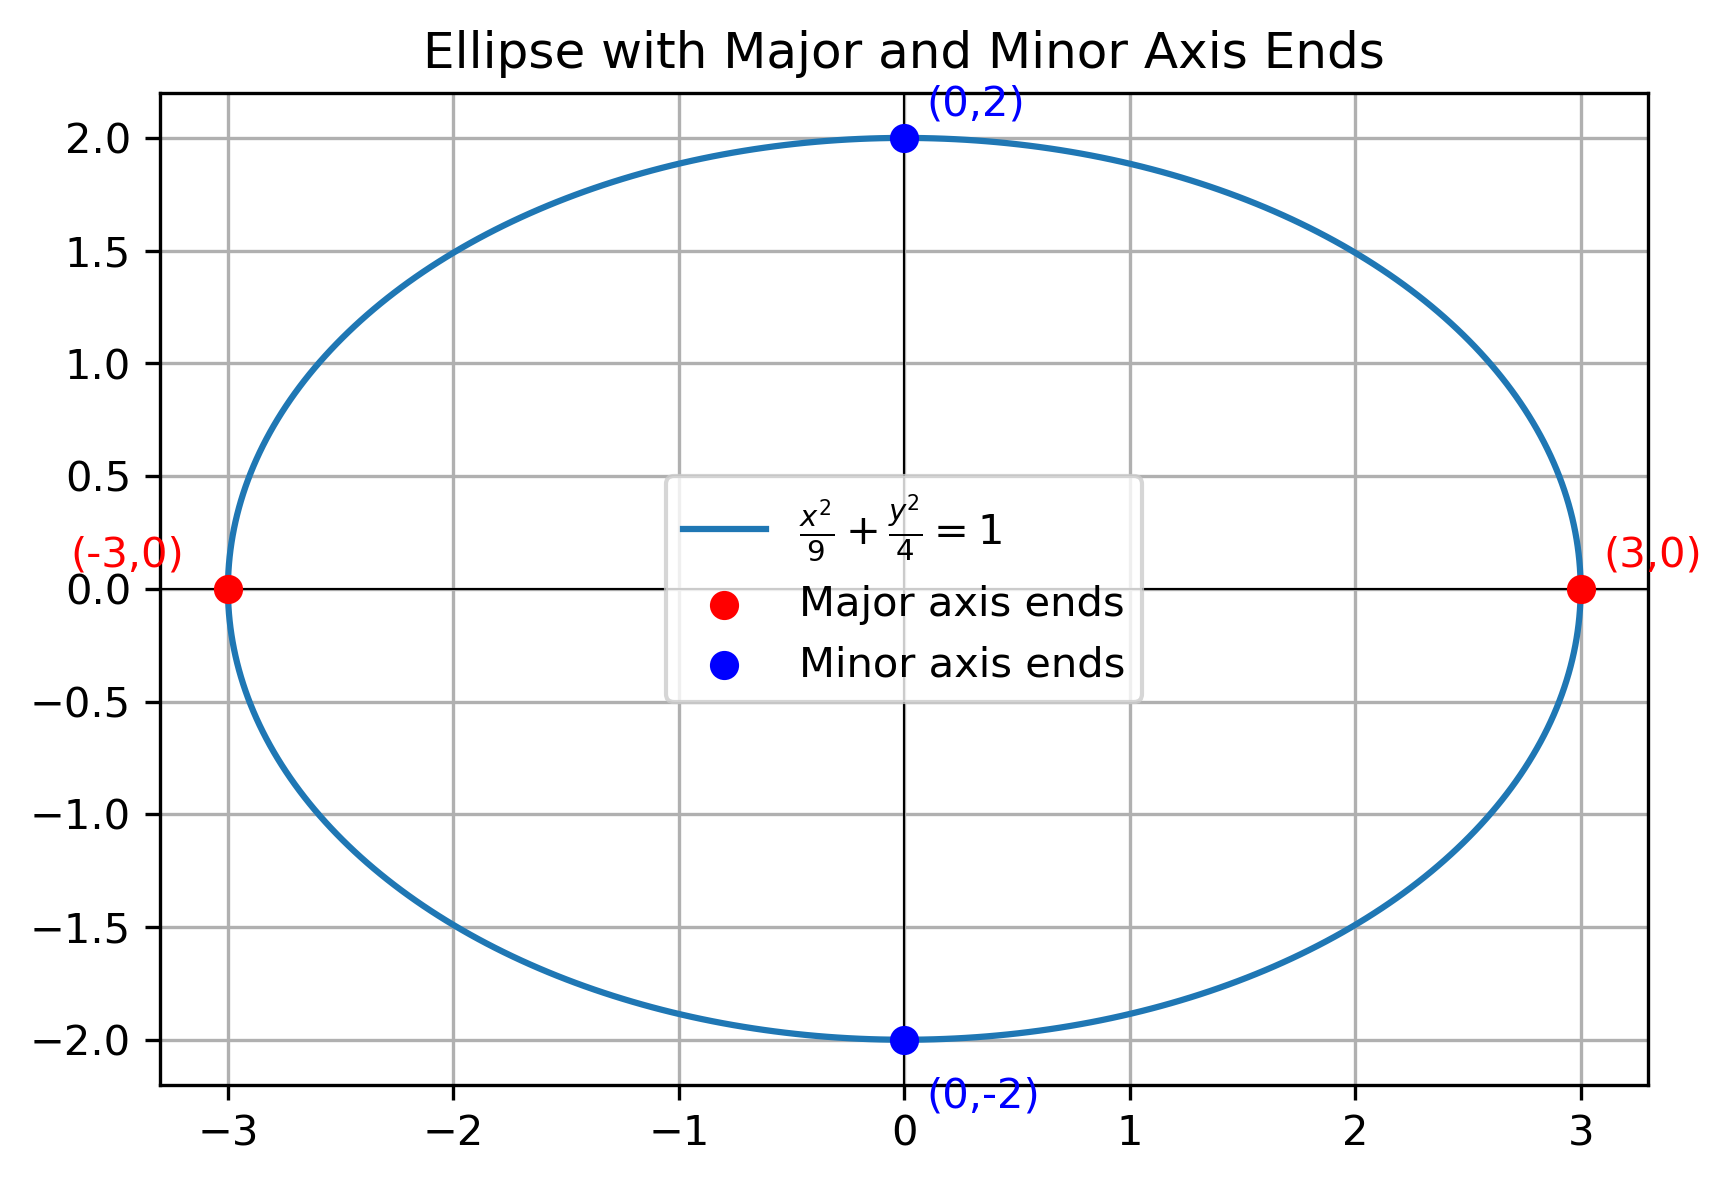
\includegraphics[width=0.9\linewidth]{figs/01.png}
    \caption{Caption}
    \label{fig:placeholder}
\end{figure}
\end{document}
